\documentclass[]{article}
\usepackage{lmodern}
\usepackage{amssymb,amsmath}
\usepackage{ifxetex,ifluatex}
\usepackage{fixltx2e} % provides \textsubscript
\ifnum 0\ifxetex 1\fi\ifluatex 1\fi=0 % if pdftex
  \usepackage[T1]{fontenc}
  \usepackage[utf8]{inputenc}
\else % if luatex or xelatex
  \ifxetex
    \usepackage{mathspec}
  \else
    \usepackage{fontspec}
  \fi
  \defaultfontfeatures{Ligatures=TeX,Scale=MatchLowercase}
\fi
% use upquote if available, for straight quotes in verbatim environments
\IfFileExists{upquote.sty}{\usepackage{upquote}}{}
% use microtype if available
\IfFileExists{microtype.sty}{%
\usepackage{microtype}
\UseMicrotypeSet[protrusion]{basicmath} % disable protrusion for tt fonts
}{}
\usepackage[margin=.9in]{geometry}
\usepackage{hyperref}
\hypersetup{unicode=true,
            pdfborder={0 0 0},
            breaklinks=true}
\urlstyle{same}  % don't use monospace font for urls
\usepackage{color}
\usepackage{fancyvrb}
\newcommand{\VerbBar}{|}
\newcommand{\VERB}{\Verb[commandchars=\\\{\}]}
\DefineVerbatimEnvironment{Highlighting}{Verbatim}{commandchars=\\\{\}}
% Add ',fontsize=\small' for more characters per line
\usepackage{framed}
\definecolor{shadecolor}{RGB}{248,248,248}
\newenvironment{Shaded}{\begin{snugshade}}{\end{snugshade}}
\newcommand{\KeywordTok}[1]{\textcolor[rgb]{0.13,0.29,0.53}{\textbf{#1}}}
\newcommand{\DataTypeTok}[1]{\textcolor[rgb]{0.13,0.29,0.53}{#1}}
\newcommand{\DecValTok}[1]{\textcolor[rgb]{0.00,0.00,0.81}{#1}}
\newcommand{\BaseNTok}[1]{\textcolor[rgb]{0.00,0.00,0.81}{#1}}
\newcommand{\FloatTok}[1]{\textcolor[rgb]{0.00,0.00,0.81}{#1}}
\newcommand{\ConstantTok}[1]{\textcolor[rgb]{0.00,0.00,0.00}{#1}}
\newcommand{\CharTok}[1]{\textcolor[rgb]{0.31,0.60,0.02}{#1}}
\newcommand{\SpecialCharTok}[1]{\textcolor[rgb]{0.00,0.00,0.00}{#1}}
\newcommand{\StringTok}[1]{\textcolor[rgb]{0.31,0.60,0.02}{#1}}
\newcommand{\VerbatimStringTok}[1]{\textcolor[rgb]{0.31,0.60,0.02}{#1}}
\newcommand{\SpecialStringTok}[1]{\textcolor[rgb]{0.31,0.60,0.02}{#1}}
\newcommand{\ImportTok}[1]{#1}
\newcommand{\CommentTok}[1]{\textcolor[rgb]{0.56,0.35,0.01}{\textit{#1}}}
\newcommand{\DocumentationTok}[1]{\textcolor[rgb]{0.56,0.35,0.01}{\textbf{\textit{#1}}}}
\newcommand{\AnnotationTok}[1]{\textcolor[rgb]{0.56,0.35,0.01}{\textbf{\textit{#1}}}}
\newcommand{\CommentVarTok}[1]{\textcolor[rgb]{0.56,0.35,0.01}{\textbf{\textit{#1}}}}
\newcommand{\OtherTok}[1]{\textcolor[rgb]{0.56,0.35,0.01}{#1}}
\newcommand{\FunctionTok}[1]{\textcolor[rgb]{0.00,0.00,0.00}{#1}}
\newcommand{\VariableTok}[1]{\textcolor[rgb]{0.00,0.00,0.00}{#1}}
\newcommand{\ControlFlowTok}[1]{\textcolor[rgb]{0.13,0.29,0.53}{\textbf{#1}}}
\newcommand{\OperatorTok}[1]{\textcolor[rgb]{0.81,0.36,0.00}{\textbf{#1}}}
\newcommand{\BuiltInTok}[1]{#1}
\newcommand{\ExtensionTok}[1]{#1}
\newcommand{\PreprocessorTok}[1]{\textcolor[rgb]{0.56,0.35,0.01}{\textit{#1}}}
\newcommand{\AttributeTok}[1]{\textcolor[rgb]{0.77,0.63,0.00}{#1}}
\newcommand{\RegionMarkerTok}[1]{#1}
\newcommand{\InformationTok}[1]{\textcolor[rgb]{0.56,0.35,0.01}{\textbf{\textit{#1}}}}
\newcommand{\WarningTok}[1]{\textcolor[rgb]{0.56,0.35,0.01}{\textbf{\textit{#1}}}}
\newcommand{\AlertTok}[1]{\textcolor[rgb]{0.94,0.16,0.16}{#1}}
\newcommand{\ErrorTok}[1]{\textcolor[rgb]{0.64,0.00,0.00}{\textbf{#1}}}
\newcommand{\NormalTok}[1]{#1}
\usepackage{graphicx,grffile}
\makeatletter
\def\maxwidth{\ifdim\Gin@nat@width>\linewidth\linewidth\else\Gin@nat@width\fi}
\def\maxheight{\ifdim\Gin@nat@height>\textheight\textheight\else\Gin@nat@height\fi}
\makeatother
% Scale images if necessary, so that they will not overflow the page
% margins by default, and it is still possible to overwrite the defaults
% using explicit options in \includegraphics[width, height, ...]{}
\setkeys{Gin}{width=\maxwidth,height=\maxheight,keepaspectratio}
\IfFileExists{parskip.sty}{%
\usepackage{parskip}
}{% else
\setlength{\parindent}{0pt}
\setlength{\parskip}{6pt plus 2pt minus 1pt}
}
\setlength{\emergencystretch}{3em}  % prevent overfull lines
\providecommand{\tightlist}{%
  \setlength{\itemsep}{0pt}\setlength{\parskip}{0pt}}
\setcounter{secnumdepth}{0}
% Redefines (sub)paragraphs to behave more like sections
\ifx\paragraph\undefined\else
\let\oldparagraph\paragraph
\renewcommand{\paragraph}[1]{\oldparagraph{#1}\mbox{}}
\fi
\ifx\subparagraph\undefined\else
\let\oldsubparagraph\subparagraph
\renewcommand{\subparagraph}[1]{\oldsubparagraph{#1}\mbox{}}
\fi

%%% Use protect on footnotes to avoid problems with footnotes in titles
\let\rmarkdownfootnote\footnote%
\def\footnote{\protect\rmarkdownfootnote}

%%% Change title format to be more compact
\usepackage{titling}

% Create subtitle command for use in maketitle
\newcommand{\subtitle}[1]{
  \posttitle{
    \begin{center}\large#1\end{center}
    }
}

\setlength{\droptitle}{-2em}
  \title{}
  \pretitle{\vspace{\droptitle}}
  \posttitle{}
  \author{}
  \preauthor{}\postauthor{}
  \date{}
  \predate{}\postdate{}

\usepackage{amssymb}
\usepackage{bm}
\usepackage{cancel}

\begin{document}

Michael Leibert

Math 504

Final Exam

~

\begin{itemize}
\item[1.] This problem aims to review several ideas - the $Ax=b$ problem, penalty methods, quadratic optimization, basis functions, positive definite matrices, projection, orthogonality - within the context of Fourier transforms.   The essential idea is that every function $f(x)$ with domain on some interval $[0,L]$ can be written in terms of an infinite number of cosine basis functions as follows:
\begin{equation*}
f(x) = \alpha_0 + \sum_{j=1}^\infty \alpha_j \cos\left(\frac{2 \pi j x}{L}\right)
\end{equation*}
where $x \in [0,L]$.   Sauer alludes to this in section $11.1$ where he discusses the discrete cosine transform.   If you want to read more, the attached notes of David Wilkins (especially see sections $8.2$ and $8.4$)  are nice.
\ 


In this problem, we will not deal with an infinite expansion, but will instead consider a basis composed of $n$ of the cosine basis functions.  Consider, as in previous homeworks, the female samples of the BoneMass dataset.  Let $N$ be the number of samples, i.e $N=259$.   Let $b_j(x) = \cos\left(2 \pi j (x - x_\text{min})/(x_\text{max} - x_\text{min})\right)$ where $x_\text{min}$ and $x_\text{max}$ are the minimum and maximum age values in the dataset.  Let $b_0(x) = 1$.  
\begin{equation*}
f(x) = \sum_{j=0}^n \alpha_j b_j(x)
\end{equation*}
\end{itemize}

~

\begin{itemize}
\item[(a)] Consider the basis functions $b_0(x), b_1(x), \dots, b_5(x)$ and let $\mathcal{F}$ be the linear function space spanned by these $6$ functions.  We have discussed orthonormal vectors, but we have not discussed orthonormal functions.   To do so, we need to introduce a norm and a dot-product on $\mathcal{F}$. The most common such dot-product is formed by integrating two functions against each other.   Specifically, let $g(x), h(x) \in \mathcal{F}$.  Then define the dot product, written $<g, h>$ by
\begin{equation*}
<g, h> = \int_{x_{\text{min}}}^{x_{\text{max}}} g(x) h(x) dx,
\end{equation*}
and the associated norm given by $\|g\|^2 = <g,g>$.  This norm is known as the $L^2$ norm.  Using this $L^2$ norm and dot-product, use numerical integration to show that the $b_i(x)$ are orthogonal and compute the coefficients necessary to normalize them.  Write your own numerical integrator.  Using numerical integration, you will find that $<b_i, b_j>$ for $i \ne j$ is small but not $0$ due to round-off error.  Explain why the value you get is small enough to be attributed to round-off error.  
\end{itemize}

~

\begin{Shaded}
\begin{Highlighting}[]
\KeywordTok{rm}\NormalTok{(}\DataTypeTok{list =} \KeywordTok{ls}\NormalTok{()); }\KeywordTok{setwd}\NormalTok{(}\StringTok{"G:}\CharTok{\textbackslash{}\textbackslash{}}\StringTok{math}\CharTok{\textbackslash{}\textbackslash{}}\StringTok{504"}\NormalTok{);}\KeywordTok{options}\NormalTok{(}\DataTypeTok{scipen=}\DecValTok{999}\NormalTok{)}
\NormalTok{bones<-}\KeywordTok{read.table}\NormalTok{(}\StringTok{"BoneMassDataF.txt"}\NormalTok{,}\DataTypeTok{header=}\NormalTok{T)}
\NormalTok{bones<-bones[}\KeywordTok{which}\NormalTok{(bones[,}\DecValTok{3}\NormalTok{] }\OperatorTok{==}\StringTok{ "female"}\NormalTok{),]}

\NormalTok{Fapprox<-}\ControlFlowTok{function}\NormalTok{(m,}\DataTypeTok{n=}\DecValTok{10000}\NormalTok{,x)\{}

\NormalTok{  MATT<-}\KeywordTok{matrix}\NormalTok{(}\DecValTok{0}\OperatorTok{:}\NormalTok{(m}\OperatorTok{-}\DecValTok{1}\NormalTok{),m,}\DecValTok{1}\NormalTok{)}

\NormalTok{  Gx<-}\ControlFlowTok{function}\NormalTok{(v,x)\{ }\ControlFlowTok{if}\NormalTok{(v }\OperatorTok{!=}\StringTok{ }\DecValTok{0}\NormalTok{) \{}
    \KeywordTok{return}\NormalTok{( }\KeywordTok{cos}\NormalTok{( (}\DecValTok{2}\OperatorTok{*}\NormalTok{pi}\OperatorTok{*}\NormalTok{v}\OperatorTok{*}\NormalTok{(x}\OperatorTok{-}\FloatTok{9.4}\NormalTok{ ) ) }\OperatorTok{/}\NormalTok{(}\FloatTok{25.55}\OperatorTok{-}\FloatTok{9.4}\NormalTok{ )) )}
\NormalTok{    \} }\ControlFlowTok{else}\NormalTok{  \{}\KeywordTok{return}\NormalTok{(}\KeywordTok{rep}\NormalTok{(}\DecValTok{1}\NormalTok{,}\KeywordTok{length}\NormalTok{(x) ))\} \}}

\NormalTok{  a=}\KeywordTok{min}\NormalTok{(x);b=}\KeywordTok{max}\NormalTok{(x)}
\NormalTok{  h=(b}\OperatorTok{-}\NormalTok{a)}\OperatorTok{/}\NormalTok{n;i=}\DecValTok{0}\OperatorTok{:}\NormalTok{(n}\OperatorTok{-}\DecValTok{1}\NormalTok{)}
\NormalTok{  W<-}\KeywordTok{apply}\NormalTok{(MATT,}\DecValTok{1}\NormalTok{,}\ControlFlowTok{function}\NormalTok{(w) }\KeywordTok{Gx}\NormalTok{(w,a}\OperatorTok{+}\NormalTok{(i}\OperatorTok{+}\DecValTok{1}\NormalTok{)}\OperatorTok{*}\NormalTok{h) )  }

\NormalTok{  Mat<-}\KeywordTok{matrix}\NormalTok{(}\OtherTok{NA}\NormalTok{,m,m)}

  \ControlFlowTok{for}\NormalTok{( i }\ControlFlowTok{in} \DecValTok{1}\OperatorTok{:}\NormalTok{m)\{}
\NormalTok{    Mat[,i] <-}\StringTok{   }\KeywordTok{colSums}\NormalTok{( (  W[  ,i ]}\OperatorTok{*}\NormalTok{W[  ,}\DecValTok{1}\OperatorTok{:}\NormalTok{m]  ) ) }\OperatorTok{*}\StringTok{ }\NormalTok{h \} }

\KeywordTok{return}\NormalTok{(Mat)}
\NormalTok{\}}

\KeywordTok{Fapprox}\NormalTok{(}\DecValTok{6}\NormalTok{,}\DataTypeTok{n=}\DecValTok{10000}\NormalTok{, bones}\OperatorTok{$}\NormalTok{age)}
\end{Highlighting}
\end{Shaded}

\begin{verbatim}
##                           [,1]                      [,2]
## [1,] 16.1499999999999985789145 -0.0000000000000002216161
## [2,] -0.0000000000000002216161  8.0749999999999992894573
## [3,] -0.0000000000000002057479 -0.0000000000000002262779
## [4,] -0.0000000000000002003689 -0.0000000000000001754460
## [5,] -0.0000000000000001406168 -0.0000000000000002019826
## [6,] -0.0000000000000002067341 -0.0000000000000002088857
##                           [,3]                      [,4]
## [1,] -0.0000000000000002057479 -0.0000000000000002003689
## [2,] -0.0000000000000002262779 -0.0000000000000001754460
## [3,]  8.0749999999999992894573 -0.0000000000000001924796
## [4,] -0.0000000000000001924796  8.0749999999999992894573
## [5,] -0.0000000000000002312535 -0.0000000000000001626260
## [6,] -0.0000000000000001361791 -0.0000000000000001532127
##                            [,5]                       [,6]
## [1,] -0.00000000000000014061682 -0.00000000000000020673407
## [2,] -0.00000000000000020198260 -0.00000000000000020888569
## [3,] -0.00000000000000023125349 -0.00000000000000013617912
## [4,] -0.00000000000000016262602 -0.00000000000000015321272
## [5,]  8.07499999999999928945726 -0.00000000000000002815026
## [6,] -0.00000000000000002815026  8.07499999999999928945726
\end{verbatim}

~

\begin{itemize} \item[]
We can see from out output matrix that the $b_i(x)$'s are orthogonal, but not orthonormal.
\end{itemize}

~

\begin{Shaded}
\begin{Highlighting}[]
\NormalTok{Gapprox<-}\ControlFlowTok{function}\NormalTok{(n,j,k,x)\{}
    
\NormalTok{    coeff<-(}\DecValTok{1}\OperatorTok{/}\KeywordTok{sqrt}\NormalTok{( }\KeywordTok{diag}\NormalTok{(}\KeywordTok{Fapprox}\NormalTok{(}\DecValTok{6}\NormalTok{,}\DataTypeTok{n=}\DecValTok{10000}\NormalTok{, bones}\OperatorTok{$}\NormalTok{age)) )) }
\NormalTok{    Fx<-}\ControlFlowTok{function}\NormalTok{(l,x)\{ }\ControlFlowTok{if}\NormalTok{(l }\OperatorTok{!=}\StringTok{ }\DecValTok{0}\NormalTok{) \{}
        \KeywordTok{return}\NormalTok{( coeff[l}\OperatorTok{+}\DecValTok{1}\NormalTok{]}\OperatorTok{*}\StringTok{ }\KeywordTok{cos}\NormalTok{( (}\DecValTok{2}\OperatorTok{*}\NormalTok{pi}\OperatorTok{*}\NormalTok{l}\OperatorTok{*}\NormalTok{(x}\OperatorTok{-}\FloatTok{9.4}\NormalTok{ ) ) }\OperatorTok{/}\NormalTok{(}\FloatTok{25.55}\OperatorTok{-}\FloatTok{9.4}\NormalTok{ )) )}
\NormalTok{        \} }\ControlFlowTok{else}\NormalTok{  \{}\KeywordTok{return}\NormalTok{( coeff[l}\OperatorTok{+}\DecValTok{1}\NormalTok{]}\OperatorTok{*}\StringTok{ }\KeywordTok{rep}\NormalTok{(}\DecValTok{1}\NormalTok{,}\KeywordTok{length}\NormalTok{(x) ))\} \}}

\NormalTok{    a=}\KeywordTok{min}\NormalTok{(x);b=}\KeywordTok{max}\NormalTok{(x)}
    
\NormalTok{    h=(b}\OperatorTok{-}\NormalTok{a)}\OperatorTok{/}\NormalTok{n;i=}\DecValTok{0}\OperatorTok{:}\NormalTok{(n}\OperatorTok{-}\DecValTok{1}\NormalTok{)}
    \KeywordTok{return}\NormalTok{(     }\KeywordTok{sum}\NormalTok{( }\KeywordTok{Fx}\NormalTok{(j,a}\OperatorTok{+}\NormalTok{(i}\OperatorTok{+}\DecValTok{1}\NormalTok{)}\OperatorTok{*}\NormalTok{h)}\OperatorTok{*}\KeywordTok{Fx}\NormalTok{(k,a}\OperatorTok{+}\NormalTok{(i}\OperatorTok{+}\DecValTok{1}\NormalTok{)}\OperatorTok{*}\NormalTok{h)}\OperatorTok{*}\NormalTok{h )    )}
\NormalTok{\}}

\NormalTok{matt<-}\KeywordTok{matrix}\NormalTok{(}\OtherTok{NA}\NormalTok{,}\DecValTok{6}\NormalTok{,}\DecValTok{6}\NormalTok{)}
\ControlFlowTok{for}\NormalTok{( J }\ControlFlowTok{in} \DecValTok{0}\OperatorTok{:}\DecValTok{5}\NormalTok{)\{}\ControlFlowTok{for}\NormalTok{( K }\ControlFlowTok{in} \DecValTok{0}\OperatorTok{:}\DecValTok{5}\NormalTok{)\{ matt[J}\OperatorTok{+}\DecValTok{1}\NormalTok{,K}\OperatorTok{+}\DecValTok{1}\NormalTok{]<-}\KeywordTok{Gapprox}\NormalTok{(}\DecValTok{10000}\NormalTok{,J,K,bones[,}\DecValTok{2}\NormalTok{]) \}\}}
\NormalTok{matt;}\KeywordTok{diag}\NormalTok{(matt )}
\end{Highlighting}
\end{Shaded}

\begin{verbatim}
##                            [,1]                       [,2]
## [1,]  1.00000000000000044408921 -0.00000000000000001931235
## [2,] -0.00000000000000001931235  0.99999999999999988897770
## [3,] -0.00000000000000001764539 -0.00000000000000002870425
## [4,] -0.00000000000000001656119 -0.00000000000000002258529
## [5,] -0.00000000000000001279359 -0.00000000000000002429968
## [6,] -0.00000000000000001767250 -0.00000000000000002429290
##                            [,3]                       [,4]
## [1,] -0.00000000000000001764539 -0.00000000000000001656119
## [2,] -0.00000000000000002870425 -0.00000000000000002258529
## [3,]  0.99999999999999988897770 -0.00000000000000002406251
## [4,] -0.00000000000000002406251  0.99999999999999988897770
## [5,] -0.00000000000000002953096 -0.00000000000000002110128
## [6,] -0.00000000000000001658829 -0.00000000000000001872282
##                             [,5]                        [,6]
## [1,] -0.000000000000000012793586 -0.000000000000000017672495
## [2,] -0.000000000000000024299681 -0.000000000000000024292905
## [3,] -0.000000000000000029530957 -0.000000000000000016588293
## [4,] -0.000000000000000021101285 -0.000000000000000018722816
## [5,]  0.999999999999999888977698 -0.000000000000000005817422
## [6,] -0.000000000000000005817422  0.999999999999999888977698
\end{verbatim}

\begin{verbatim}
## [1] 1 1 1 1 1 1
\end{verbatim}

~

\begin{itemize} \item[]
We have computed the coefficients necessary to normalize them.

\  


Error for Riemann integration:
 
 \begin{align*}
     \text{error} &= \left| \int_a^{a+h} f(x) \ \text{d}x - f(a)\cdot h \right| \\
     &\approx \left| \int_a^{a+h} \Big( f(a) + f'(a)(x-a) \Big) \ \text{d}x - f(a)\cdot h \right| \\
     &=\left| f(a) \cdot h +  f'(a) \cfrac{(x-a)^2}{2} \  \bigg|_a^{a+h}  - f(a)\cdot h  \right| \\
     &= f'(a)  \cfrac{h^2}{2} \\
     & \approx h^2 \text{ (error for one rectangle) }
 \end{align*}
 
  Riemann integration has an error of roughly $\left(h^2\right) \left(\cfrac{b-a}{h}\right) = (b-a)\cdot h$, where $h$ is the grid width.
  
  \ 
  
  The total error is about 0.02608486 so we can attribute the error we are getting to roundoff error.
\end{itemize}

~

~

\begin{itemize}
\item[(b)] Continuing from (a), find $f(x) \in \mathcal{F}$ that best fits the data using least squares as the loss function.  Justify each step in your computation.  Plot the data and resulting fit.   Explain how determining $f(x)$ corresponds to (i) a linear regression (ii) projection of a vector onto a linear space (iii) quadratic optimization.
\end{itemize}

~

\begin{itemize} \item[] 
In this step, I am writing a function for any general $b_j$. If \text{w} is 1,...,5, I obtain the normalizing coefficients, apply them to the $b_j = 1,...,5$, and return the specified $b_j$. If 0 is given I return 1's. 
\end{itemize}

~

\begin{Shaded}
\begin{Highlighting}[]
\NormalTok{Fx<-}\ControlFlowTok{function}\NormalTok{(w,x)\{   }
    \CommentTok{#need this matrix for the normalizing Coefficients}
\NormalTok{    ncoef<-(}\DecValTok{1}\OperatorTok{/}\KeywordTok{sqrt}\NormalTok{( }\KeywordTok{diag}\NormalTok{(}\KeywordTok{Fapprox}\NormalTok{(}\DecValTok{6}\NormalTok{,}\DataTypeTok{n=}\DecValTok{10000}\NormalTok{, bones}\OperatorTok{$}\NormalTok{age)) )) }
    \ControlFlowTok{if}\NormalTok{(w }\OperatorTok{==}\StringTok{ }\DecValTok{0}\NormalTok{ ) \{}\KeywordTok{return}\NormalTok{(   }\KeywordTok{rep}\NormalTok{(}\DecValTok{1}\NormalTok{,}\KeywordTok{length}\NormalTok{(x) ))  \} }\ControlFlowTok{else}\NormalTok{ \{}
    \KeywordTok{return}\NormalTok{( ncoef[w}\OperatorTok{+}\DecValTok{1}\NormalTok{]}\OperatorTok{*}\StringTok{ }\KeywordTok{cos}\NormalTok{( (}\DecValTok{2}\OperatorTok{*}\NormalTok{pi}\OperatorTok{*}\NormalTok{w}\OperatorTok{*}\NormalTok{(x}\OperatorTok{-}\FloatTok{9.4}\NormalTok{ ) ) }\OperatorTok{/}\NormalTok{(}\FloatTok{25.55}\OperatorTok{-}\FloatTok{9.4}\NormalTok{ )) )}
\NormalTok{        \} \}}
\end{Highlighting}
\end{Shaded}

~

\begin{itemize} \item[] 
In this step I form the model matrix. By using our function \text{Fx} above. Then I solve for $\alpha$.
\end{itemize}

~

\begin{Shaded}
\begin{Highlighting}[]
\NormalTok{model_matrix <-}\StringTok{ }\ControlFlowTok{function}\NormalTok{(x,m) \{ }
\NormalTok{    nx <-}\StringTok{ }\KeywordTok{length}\NormalTok{(x)}
\NormalTok{    A<-}\KeywordTok{matrix}\NormalTok{(}\OtherTok{NA}\NormalTok{,nx,m}\OperatorTok{+}\DecValTok{1}\NormalTok{)}
    \ControlFlowTok{for}\NormalTok{( i }\ControlFlowTok{in} \DecValTok{0}\OperatorTok{:}\NormalTok{m)\{     A[,(i}\OperatorTok{+}\DecValTok{1}\NormalTok{)] <-}\StringTok{ }\KeywordTok{Fx}\NormalTok{(i,x)  \}}
    \KeywordTok{colnames}\NormalTok{(A )<-}\OtherTok{NULL}\NormalTok{; }\KeywordTok{return}\NormalTok{(A)   \}}
\NormalTok{B<-}\StringTok{ }\KeywordTok{model_matrix}\NormalTok{(bones}\OperatorTok{$}\NormalTok{age,}\DecValTok{5}\NormalTok{)}
\NormalTok{Alpha <-}\StringTok{ }\KeywordTok{solve}\NormalTok{(}\KeywordTok{t}\NormalTok{(B) }\OperatorTok\StringTok{ }\NormalTok{B , }\KeywordTok{t}\NormalTok{(B) }\OperatorTok\StringTok{ }\KeywordTok{as.matrix}\NormalTok{(bones[,}\DecValTok{4}\NormalTok{])) }
\end{Highlighting}
\end{Shaded}

\begin{Shaded}
\begin{Highlighting}[]
\NormalTok{x_grid <-}\StringTok{ }\KeywordTok{seq}\NormalTok{(}\KeywordTok{min}\NormalTok{(bones}\OperatorTok{$}\NormalTok{age), }\KeywordTok{max}\NormalTok{(bones}\OperatorTok{$}\NormalTok{age), .}\DecValTok{01}\NormalTok{)}
\NormalTok{B_grid <-}\StringTok{ }\KeywordTok{model_matrix}\NormalTok{(x_grid,}\DecValTok{5}\NormalTok{); y_grid <-}\StringTok{ }\NormalTok{B_grid }\OperatorTok\StringTok{ }\NormalTok{Alpha}
\end{Highlighting}
\end{Shaded}

\begin{Shaded}
\begin{Highlighting}[]
\KeywordTok{par}\NormalTok{(}\DataTypeTok{mar=}\KeywordTok{c}\NormalTok{(}\FloatTok{4.1}\NormalTok{,}\FloatTok{4.1}\NormalTok{,}\DecValTok{2}\NormalTok{,}\DecValTok{1}\NormalTok{))}
\KeywordTok{plot}\NormalTok{(bones}\OperatorTok{$}\NormalTok{age, bones[,}\DecValTok{4}\NormalTok{], }\DataTypeTok{ylim=}\KeywordTok{c}\NormalTok{(}\KeywordTok{min}\NormalTok{(bones[,}\DecValTok{4}\NormalTok{])}\OperatorTok{-}\NormalTok{.}\DecValTok{02}\NormalTok{,}\KeywordTok{max}\NormalTok{(bones[,}\DecValTok{4}\NormalTok{]) }\OperatorTok{+}\StringTok{ }\NormalTok{.}\DecValTok{02}\NormalTok{) )}
\KeywordTok{lines}\NormalTok{(x_grid, y_grid, }\DataTypeTok{col=}\StringTok{"red"}\NormalTok{, }\DataTypeTok{lwd=}\DecValTok{2}\NormalTok{)   }
\end{Highlighting}
\end{Shaded}

\includegraphics{504FINAL_files/figure-latex/unnamed-chunk-6-1.pdf}

~

\begin{itemize} \item[] 
We have some data, $x^{(i)} \in \mathbb{R}$ and $y_i \in \mathbb{R}$, and we wish to approximate $y$ by a function $f(x)$, when $f(x) \in \mathcal{F}$ and $f(x): \mathbb{R}^n \rightarrow \mathbb{R}$.

\ 

Let $\mathcal{F}$ be:


\begin{equation*} 
\mathcal{F} = \{ f(x): f(x): \mathbb{R}^n \rightarrow \mathbb{R}, f(x) = 5^{th} \text{ harmonic} \} . 
\end{equation*}


We use least squares to find the $f(x) \in \mathcal{F}$

\begin{align}
     \min\limits_{f(x) \in \mathcal{F} } \sum\limits_{i=1}^N \left| y_i - f\left(x^{(i)} \right) \right|
\end{align} 
 
 
 It is key to note that $\mathcal{F}$ is a linear function / vector space. It is true that for any $g(x) \in \mathcal{F}$ and $h(x) \in \mathcal{F}$, $c_1 g(x) + c_2 h(x) \in \mathcal{F}$, where $c_1,c_2 \in \mathbb{R}$
 
 \ 
 
 
 Our function $f(x)$ can be written as:
 
 \ 
 
\begin{align*} f(x) &= \sum_{j=0}^n \alpha_j b_j(x) = \alpha_0 (1) + \alpha_1 \cos\left(
    \cfrac{2\pi(1)\left(x-x_{max}\right)}{\left(x_{max}-x_{min}\right)} \right) + ...  + \alpha_5 \cos\left(
    \cfrac{2\pi(5)\left(x-x_{max}\right)}{\left(x_{max}-x_{min}\right)} \right) 
    \end{align*} 
 
 \ 
 
 so we can rewrite (1) as:
 
\ 

\hspace{-1 cm}
\begin{align}
     \min\limits_{f(x) \in \mathcal{F} } \sum\limits_{i=1}^N \left| y_i - f\left(x^{(i)} \right) \right| =
     \min\limits_{\alpha \in \mathbb{R}^6 } \sum\limits_{i=1}^N \left|\alpha_0 + \alpha_1 \cos\left(
    \cfrac{2\pi\left(x_i-x_{max}\right)}{\left(x_{max}-x_{min}\right)} \right) + ...  + \alpha_5 \cos\left(
    \cfrac{10\pi\left(x_i-x_{max}\right)}{\left(x_{max}-x_{min}\right)} \right)  \right|^2_{\text{ .} }
\end{align}
 
 \ 

 The sum in the RHS of (2) can be put into matrix form:
 
 \begin{align}
     \begin{pmatrix} y_1 \\ y_2 \\ \vdots \\ y_N \\[.25 em]  \end{pmatrix} -
      \begin{pmatrix}
        \\[-.75em]
        b_0\left(x^{(1)}\right) & b_1\left(x^{(1)}\right) & ... &  b_5\left(x^{(1)}\right)   \\[.5em]
        b_0\left(x^{(2)}\right) & b_1\left(x^{(2)}\right) & ...  & b_5\left(x^{(2)}\right)  \\[.5em]
        \vdots & \vdots & \ddots & \vdots  \\[.5em]
        b_0\left(x^{(N)}\right) & b_1\left(x^{(N)}\right) &...  &  b_5\left(x^{(N)}\right)   \\[.5em]
        \end{pmatrix}
        \begin{pmatrix} \alpha_1 \\ \alpha_2 \\ \vdots \\ \alpha_N \\[.25 em]  \end{pmatrix}
 \end{align}

\ 

and (2) is equivalent to 


\begin{align}
    \min\limits_{\alpha \in \mathbb{R}^6 } ||{\bm y}-B{\bm \alpha}||^2. 
\end{align}
 \end{itemize}

\begin{itemize} \item[ ] 
So given some data we are trying to fit through that data the best $5^{th}$ harmonic. We are not doing regression in the sense of fitting a line because we are fitting a $5^{th}$ harmonic. But we end up doing the same exact thing that we do for linear regression (minimize sum of squares, replace with model matrix).


\ 




The important part of linear regression is not that the functions are linear, it is that the space of the functions we are considering are a linear function space. We are still linear in the parameters. Thus in this context, determining $f(x)$ corresponds to a linear regression.


\ 

 Now for projection consider the ${\bm y}$, $B$ and ${\bm \alpha}$ from (3) above. We wish to choose ${\bm \alpha}$ so that $B{\bm \alpha}$ is as close as possible to ${\bm y}$. Or put another way, find the point in the $\text{Span}(B) = \text{Span}\left(b^{(0)} \ \ b^{(1)} \ \ \dots \ \ b^{(5)}\right)$ closest to ${\bm y}$. If $n=2$, we would have a visual like this:
\end{itemize}

~

\hfil 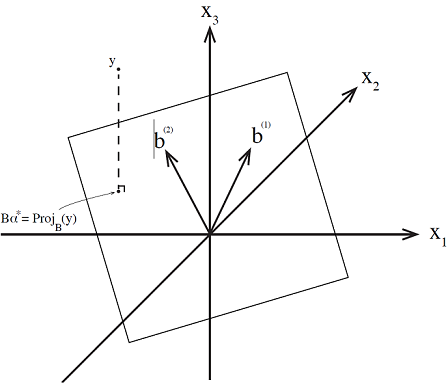
\includegraphics{proj2.png}

~

\begin{itemize} \item[ ] 
For $n=6$, $b_{0}$ through $b_{5}$ are linearly combining to form a plane Again, we want to find the point closest to ${\bm y}$. It will be the point that is orthogonal and this point will be the $\text{Proj}_B(y)$.
\end{itemize}

~

\begin{itemize} \item[ ] 
The projection of $x \in \mathbb{R}$ onto $\Omega$ is the closest point in $\Omega$ to $x$.
\end{itemize}

\begin{align*}
    P_\Omega(x) = \min_{z \in \Omega} ||z-x||
\end{align*}

\begin{itemize} \item[ ] 
Now suppose $\Omega =  \text{Span}\left(b^{(0)} \ \ b^{(1)} \ \ \dots \ \ b^{(5)}\right)$, and \(\displaystyle P_\Omega(x) = \min_{z \in \Omega} ||z-y|| \), where 
\end{itemize}

\begin{align*}
     z &= \alpha_0 b^{(0)} + \alpha_1 b^{(1)} + ... + \alpha_5 b^{(5)} = B{\bm \alpha} = 
        \begin{pmatrix}
         b^{(0)} &  b^{(1)}& \dots & b^{(5)}
        \end{pmatrix}
        \begin{pmatrix}
        \alpha_0 & \alpha_1 & \dots & \alpha_5
        \end{pmatrix}^T
\end{align*}\begin{itemize} \item[ ] 
and 
\end{itemize}\begin{align} \min_{z \in \Omega} ||z-y|| = \min_{z \in \Omega} ||\alpha_0 b^{(0)} + \alpha_1 b^{(1)} + ... + \alpha_5 b^{(5)}-y|| \end{align}

\begin{itemize} \item[ ] 
So we have $\min\limits_{\alpha \in \mathbb{R}} ||B \alpha - y||^2$. To tie projection and linear regression together, we can view linear regression as a projection onto the span of the columns of the model matrix. 
\end{itemize}

~

\begin{itemize} \item[ ] 
Now tying both of them to quadratic optimization. When we have a linear subspace and project onto it, it leads to a minimization of a quadratic $\min\limits_{\alpha \in \mathbb{R}^6} ||B{\bm \alpha}-{\bm y}||^2$, (5) above. When $\mathcal{F}$ is a linear function space then the regression is a minimization of a quadratic $\min\limits_{\alpha \in \mathbb{R}^6 } ||{\bm y}-B{\bm \alpha}||^2$, (4) above.
\end{itemize}

~

\begin{itemize} \item[ ] 
Both (4) and (5) are solved with the normal equations. 
\end{itemize}

\begin{align*}
L(\alpha) &= \sum_{i=1}^N \left(   y_i - \alpha_0 + \alpha_1x_1^{(i)} + \alpha_2x_2^{(i)} + ... \alpha_nx_n^{(i)}  \right)^2 \\
&= \sum_{i=1}^N r_i^2 \\
&= {\bf r}\cdot{\bf r} \\
&=\left(y-B \alpha \right) \cdot \left(y-B \alpha\right) \\
&=\left(y-B \alpha\right)^T \left(y-B \alpha\right) \\
&= \left(y^T- (B \alpha)^T \right) \left(y-B \alpha\right) \\
&=y^Ty - (B\alpha)^Ty-y^TB\alpha + (B \alpha)^T B \alpha \\
&= y^Ty - 2(B^T y )^T  \alpha +\alpha^T B^T B \alpha \\
\\
\nabla L(\alpha) &= -\cfrac{1}{2} \left(B^T B \right)^{-1} \left(-2B^T y \right) \\
&= \left( B^T B \right)^{-1} B^T y
\end{align*}

\begin{itemize} \item[ ] 
We have shown that determining $f(x)$ corresponds to a linear regression, projection of a vector onto a linear space, and a quadratic optimization.
\end{itemize}

~

\begin{itemize}
\item[(c)] Consider $\mathcal{F}$, but now formed from all $b_i(x)$ with $i=0,1,\dots,1000$.  Show that the best fit is now not unique.  Construct a penalty term that penalizes $f(x)$ (or equivalently $\alpha$) for contributions from $b_j(x)$ with large $j$.  Show that your penalty term creates a unique best fit $f(x)$ for any penalty value $\rho > 0$.  (Recall, you can do this by showing that the penalty term corresponds to a positive definite matrix.  Go through the argument).  What happens to the fit as $\rho$ increases?   Show plots of the data and fit for different $\rho$.  
\end{itemize}

~

\begin{itemize} \item[ ] 
 We have an underdetermined system, more variables than equations. There cannot be more basic variables than there are equations, so there must be at least one free variable. Such a variable may be assigned infinitely many different values. Because our system is consistent (has at least one solution), each different value of a free variable will produce a different solution. 
\end{itemize}

~

\begin{itemize}    \item[] 

We note, $\alpha = \left( B^TB+\rho \ \Omega \right)^{-1}$ is a unique minimum. If $\rho$ is 0, $B^TB$ will not be invertible because $B$ is a fat matrix and there are some values $B$ takes to 0.

\ 

If $\rho>0$ we get a unique solution and $B^TB+\rho \Omega$ can be inverted. Both are $B^TB$ and $\rho \ \Omega$ are positive semidefinite matrices.

\ 

\hfil \( \displaystyle v^T(B^TB)v \geq 0 \) and \( \displaystyle v^T(\rho \ \Omega)v \geq 0\) 

\ 

For any $\alpha$, $\alpha^TB^TB\alpha = ||B\alpha||^2 > 0$. We also know,

\ 

\hfil \(\displaystyle \alpha^T \Omega \alpha = \int_{x_{min}}^{x_{max}} \left( \left[ \sum_j \alpha_j b_j(z) \right]'' \right)^2 \text{d}z. \)

\ 

\ 

The integral is non-negative since the integrand is square, so $\alpha^T \Omega \alpha \geq 0$. The only way $\alpha^T \Omega \alpha = 0$ is if 

\ 

\hfil \( \displaystyle \sum_j \alpha_j b_j(z) \)

\ 

has a second derivative that is zero for all $z$, that is the function is linear. 

\ 

If $\alpha$ is such that \( \displaystyle \sum_j \alpha_j b_j(z) \) is not linear, then $\alpha^T \Omega \alpha  > 0$, and we can conclude $\alpha^t \left(B^TB+\rho \Omega\right) \alpha >0$, which in turn gives $\left(B^TB+\rho \Omega \right)\alpha \neq 0$.

\ 


If $\alpha$ is such that \( \displaystyle \sum_j \alpha_j b_j(z) \) is linear, then $\alpha^T \Omega \alpha  = 0$. However, the $i$th coordinate of the vector $B\alpha$, is given by
 

\hfil \( \displaystyle \sum_j \alpha_j b_j(x_i) \),
 

where $x_i$ is the $i$th sample. If $B\alpha = 0$, then the function \( \displaystyle \sum_j \alpha_j b_j(z) \) is a linear function that is zero at all $x_i$. But this means the function is zero and hence $\alpha=0$. 

\ 

This allows us to conclude that if $\alpha^T\Omega\alpha = 0$ and $\alpha \neq 0$, then $B\alpha\neq0$ and therefore $\alpha^TB^TB\alpha> 0$. We can also conclude that in this case $\left(B^TB+\rho \Omega \right)\alpha \neq 0$.

\ 

Therefore, for either of the two cases when $\sum_j \alpha_j b_j(z)$ is linear or not linear, we have shown that for any $\alpha \neq 0$ we have $\left(B^TB+\rho \Omega \right)\alpha \neq 0$, so $B^TB+\rho \  \Omega$ is invertible.
\end{itemize}

~

\begin{Shaded}
\begin{Highlighting}[]
\NormalTok{Fx<-}\ControlFlowTok{function}\NormalTok{(w,x)\{   }
    \CommentTok{#need this matrix for the normalizing Coefficients}
\NormalTok{    ncoef<-(}\DecValTok{1}\OperatorTok{/}\KeywordTok{sqrt}\NormalTok{( }\KeywordTok{diag}\NormalTok{(}\KeywordTok{Fapprox}\NormalTok{(}\DecValTok{1001}\NormalTok{,}\DataTypeTok{n=}\DecValTok{10000}\NormalTok{, bones}\OperatorTok{$}\NormalTok{age)) )) }
    \ControlFlowTok{if}\NormalTok{(w }\OperatorTok{==}\StringTok{ }\DecValTok{0}\NormalTok{ ) \{}\KeywordTok{return}\NormalTok{(   }\KeywordTok{rep}\NormalTok{(}\DecValTok{1}\NormalTok{,}\KeywordTok{length}\NormalTok{(x) ))  \} }\ControlFlowTok{else}\NormalTok{ \{}
    \KeywordTok{return}\NormalTok{( ncoef[w}\OperatorTok{+}\DecValTok{1}\NormalTok{]}\OperatorTok{*}\StringTok{ }\KeywordTok{cos}\NormalTok{( (}\DecValTok{2}\OperatorTok{*}\NormalTok{pi}\OperatorTok{*}\NormalTok{w}\OperatorTok{*}\NormalTok{(x}\OperatorTok{-}\FloatTok{9.4}\NormalTok{ ) ) }\OperatorTok{/}\NormalTok{(}\FloatTok{25.55}\OperatorTok{-}\FloatTok{9.4}\NormalTok{ )) )}
\NormalTok{        \} \}}
\NormalTok{dmat<-}\ControlFlowTok{function}\NormalTok{(m,}\DataTypeTok{n=}\DecValTok{10000}\NormalTok{,x)\{}

\NormalTok{MATT<-}\KeywordTok{matrix}\NormalTok{(}\DecValTok{0}\OperatorTok{:}\NormalTok{(m}\OperatorTok{-}\DecValTok{1}\NormalTok{),m,}\DecValTok{1}\NormalTok{)}

\NormalTok{dFx<-}\ControlFlowTok{function}\NormalTok{(v,x)\{ }\ControlFlowTok{if}\NormalTok{(v }\OperatorTok{!=}\StringTok{ }\DecValTok{0}\NormalTok{) \{}
    \KeywordTok{return}\NormalTok{( }\OperatorTok{-}\NormalTok{((}\DecValTok{4}\OperatorTok{*}\NormalTok{pi}\OperatorTok{^}\DecValTok{2}\OperatorTok{*}\NormalTok{v}\OperatorTok{^}\DecValTok{2}\NormalTok{)}\OperatorTok{/}\NormalTok{(}\FloatTok{16.15}\OperatorTok{^}\DecValTok{2}\NormalTok{))}\OperatorTok{*}\StringTok{ }\KeywordTok{cos}\NormalTok{( (}\DecValTok{2}\OperatorTok{*}\NormalTok{pi}\OperatorTok{*}\NormalTok{v}\OperatorTok{*}\NormalTok{(x}\OperatorTok{-}\FloatTok{9.4}\NormalTok{ ))}\OperatorTok{/}\FloatTok{16.15}\NormalTok{)}
\NormalTok{    )   \} }\ControlFlowTok{else}\NormalTok{  \{}\KeywordTok{return}\NormalTok{(}\KeywordTok{rep}\NormalTok{(}\DecValTok{1}\NormalTok{,}\KeywordTok{length}\NormalTok{(x) ))\} \}}

\NormalTok{a=}\KeywordTok{min}\NormalTok{(x);b=}\KeywordTok{max}\NormalTok{(x)}
\NormalTok{h=(b}\OperatorTok{-}\NormalTok{a)}\OperatorTok{/}\NormalTok{n;i=}\DecValTok{0}\OperatorTok{:}\NormalTok{(n}\OperatorTok{-}\DecValTok{1}\NormalTok{)}
\NormalTok{W<-}\KeywordTok{apply}\NormalTok{(MATT,}\DecValTok{1}\NormalTok{,}\ControlFlowTok{function}\NormalTok{(w) }\KeywordTok{dFx}\NormalTok{(w,a}\OperatorTok{+}\NormalTok{(i}\OperatorTok{+}\DecValTok{1}\NormalTok{)}\OperatorTok{*}\NormalTok{h) )  }
\NormalTok{\}}

\NormalTok{Bpp<-}\KeywordTok{dmat}\NormalTok{(}\DecValTok{1000}\OperatorTok{+}\DecValTok{1}\NormalTok{,}\DataTypeTok{n=}\DecValTok{10000}\NormalTok{, bones}\OperatorTok{$}\NormalTok{age)}
\NormalTok{z<-}\KeywordTok{seq}\NormalTok{(}\KeywordTok{min}\NormalTok{(bones}\OperatorTok{$}\NormalTok{age),}\KeywordTok{max}\NormalTok{(bones}\OperatorTok{$}\NormalTok{age),   }\DataTypeTok{length.out =} \DecValTok{10000}\NormalTok{ )}
\NormalTok{h<-z[}\DecValTok{2}\NormalTok{]}\OperatorTok{-}\NormalTok{z[}\DecValTok{1}\NormalTok{]}


\NormalTok{omega<-h}\OperatorTok{*}\NormalTok{(}\KeywordTok{t}\NormalTok{(Bpp) }\OperatorTok\StringTok{ }\NormalTok{Bpp )  }\CommentTok{#Penalty Term}

\NormalTok{B<-}\StringTok{ }\KeywordTok{model_matrix}\NormalTok{(bones}\OperatorTok{$}\NormalTok{age,}\DecValTok{1000}\NormalTok{)}
\NormalTok{n=}\DecValTok{1001}
\NormalTok{y<-}\KeywordTok{as.matrix}\NormalTok{( bones[,}\DecValTok{4}\NormalTok{] )}
\NormalTok{A<-}\KeywordTok{matrix}\NormalTok{(}\OtherTok{NA}\NormalTok{,(n ),}\DecValTok{3}\NormalTok{)}
\NormalTok{A[,}\DecValTok{1}\NormalTok{]<-}\KeywordTok{solve}\NormalTok{( }\KeywordTok{t}\NormalTok{(B)}\OperatorTok\NormalTok{B }\OperatorTok{+}\StringTok{ }\NormalTok{(.}\DecValTok{0001} \OperatorTok{*}\StringTok{ }\NormalTok{omega) ) }\OperatorTok\StringTok{ }\KeywordTok{t}\NormalTok{(B)}\OperatorTok\StringTok{ }\NormalTok{y}
\NormalTok{A[,}\DecValTok{2}\NormalTok{]<-}\KeywordTok{solve}\NormalTok{( }\KeywordTok{t}\NormalTok{(B)}\OperatorTok\NormalTok{B }\OperatorTok{+}\StringTok{ }\NormalTok{(}\DecValTok{1} \OperatorTok{*}\StringTok{ }\NormalTok{omega) ) }\OperatorTok\StringTok{ }\KeywordTok{t}\NormalTok{(B)}\OperatorTok\StringTok{ }\NormalTok{y}
\NormalTok{A[,}\DecValTok{3}\NormalTok{]<-}\KeywordTok{solve}\NormalTok{( }\KeywordTok{t}\NormalTok{(B)}\OperatorTok\NormalTok{B }\OperatorTok{+}\StringTok{ }\NormalTok{(}\DecValTok{100} \OperatorTok{*}\StringTok{ }\NormalTok{omega) ) }\OperatorTok\StringTok{ }\KeywordTok{t}\NormalTok{(B)}\OperatorTok\StringTok{ }\NormalTok{y}


\KeywordTok{par}\NormalTok{(}\DataTypeTok{mar=}\KeywordTok{c}\NormalTok{(}\FloatTok{4.1}\NormalTok{,}\FloatTok{4.1}\NormalTok{,}\DecValTok{1}\NormalTok{,}\DecValTok{1}\NormalTok{))}
\NormalTok{datt<-}\KeywordTok{data.frame}\NormalTok{(bones}\OperatorTok{$}\NormalTok{age, B}\OperatorTok\StringTok{ }\NormalTok{A[,}\DecValTok{1}\NormalTok{], B}\OperatorTok\StringTok{ }\NormalTok{A[,}\DecValTok{2}\NormalTok{], B}\OperatorTok\StringTok{ }\NormalTok{A[,}\DecValTok{3}\NormalTok{] )}
\NormalTok{datt<-datt[}\KeywordTok{with}\NormalTok{(datt, }\KeywordTok{order}\NormalTok{(bones}\OperatorTok{$}\NormalTok{age)), ]}

\KeywordTok{plot}\NormalTok{(bones[,}\DecValTok{2}\NormalTok{], bones[,}\DecValTok{4}\NormalTok{], }\DataTypeTok{xlab=}\StringTok{"age"}\NormalTok{, }\DataTypeTok{ylab=}\StringTok{"spnbmd"}\NormalTok{)}
\KeywordTok{lines}\NormalTok{( datt[,}\DecValTok{1}\NormalTok{],datt[,}\DecValTok{2}\NormalTok{],}\DataTypeTok{col=}\StringTok{"red"}\NormalTok{, }\DataTypeTok{lwd=}\DecValTok{2}\NormalTok{)}
\KeywordTok{lines}\NormalTok{( datt[,}\DecValTok{1}\NormalTok{],datt[,}\DecValTok{3}\NormalTok{],}\DataTypeTok{col=}\StringTok{"blue"}\NormalTok{, }\DataTypeTok{lwd=}\DecValTok{2}\NormalTok{)}
\KeywordTok{lines}\NormalTok{( datt[,}\DecValTok{1}\NormalTok{],datt[,}\DecValTok{4}\NormalTok{],}\DataTypeTok{col=}\StringTok{"green"}\NormalTok{, }\DataTypeTok{lwd=}\DecValTok{2}\NormalTok{)}
\end{Highlighting}
\end{Shaded}

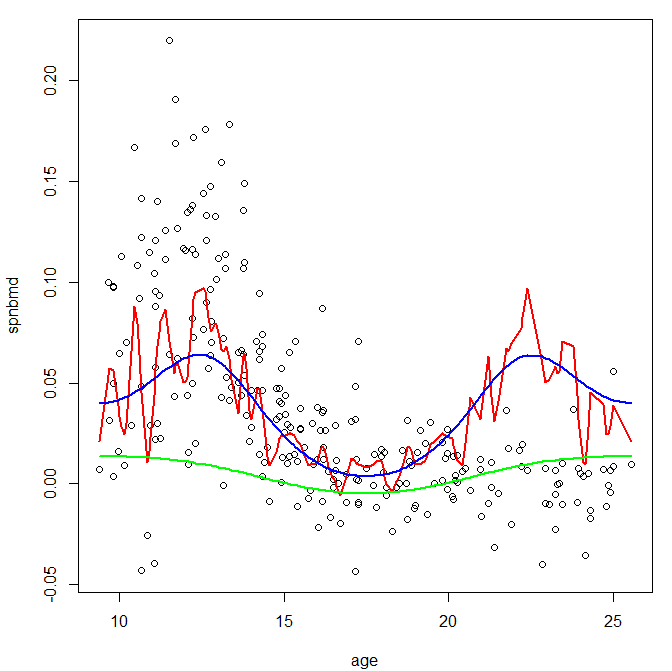
\includegraphics{penal.png}

\begin{itemize} \item[ ] 
As $\rho$ increases the regression becomes more linear in order to reduce the penalty term, the result is that the fitting term increases, meaning that the fit becomes poorer.
\end{itemize}

\newpage

\begin{itemize} \item[(2)] This problem repeats the neural net problem of hw $12$, but using Martens' conjugate gradient method. You will apply his Algorithm 1, although with some differences.  As we discussed in class, let $f(\eta)$ be the \textbf{negative} log-likelihood function (negative, so we can minimize rather than maximize).  Martens' uses $\theta$ for the net parameters, but to connect to our notation, I will use $\eta$.
\end{itemize}

~

\begin{itemize} \item[(a)] 
In Algorithm $1$, Martens defines $B = Hf(\eta) + \lambda I$.  Explain why Martens adds a $\lambda I$.  (This connects to our discussion of Hessian modification.)   Martens changes $\lambda$ at every iteration of the optimization as he discusses in Section $4.1$.   Here, let's take a simplified approach.  Let $\eta^{(i)}$ and $\eta^{(i+1)}$ be the $i$th and $i+1$th values of $\eta$ in the optimizatio iteration.  If the algorithm has made good progress in iteration $i+1$ relative to $\eta^{(i)}$, then lower $\lambda$.  If the algorithm has made poor progress, then raise $\lambda$.  It is up to you to define good/poor and to determine how much to lower/raise $\lambda$.   Explain why we should raise $\lambda$ if the progress is poor.
\end{itemize}

~

\begin{itemize} \item[ ] 
 The neural net is a nonconvex optimization, we may go to a local minimum. We want the hessian of the negative log likelihood to be positive definite, or alternatively we want all the eigenvalues to be positive. However, for neural nets the hessian of negative log likelihood is not going to be positive definite because it is not a convex function. 
 
 \ 
 
 However we can modify the hessian such that it is positive definite and similar to the hessian. We can rewrite the hessian as a decomposition, and add a constant so the minimum eigenvalue becomes positive
 
 \begin{align*}
     H&= Q \begin{pmatrix}
     \lambda_1  & &  \\
     & \lambda_2 &  \\
     & & \ddots &  \\
       &  &  &\lambda_n
     \end{pmatrix} Q^T \\
     \\
     H + \lambda I &= Q \begin{pmatrix}
     \lambda_1 + \lambda  & &  \\
     & \lambda_2 + \lambda&  \\
     & & \ddots &  \\
       &  &  &\lambda_n +  \lambda
     \end{pmatrix} Q^T \\
     \\
     &= Q \begin{pmatrix}
     \lambda_1  & &  \\
     & \lambda_2 &  \\
     & & \ddots &  \\
       &  &  &\lambda_n
     \end{pmatrix} Q^T+
     Q \begin{pmatrix}
     \lambda  & &  \\
     & \lambda &  \\
     & & \ddots &  \\
       &  &  &\lambda
     \end{pmatrix} Q^T.
 \end{align*}
 
We should raise $\lambda$ if we are doing poorly, because raising the lambdas enough will get all of our eigenvalues positive. When the eigenvalues are all positive we are in a region of the function that is locally convex and we will go down.
\end{itemize}

~

\begin{itemize} \item[(b)] 
Martens' points out that conjugate gradient does not require actually computing $Hf(\eta)$, but rather being able to compute $Hf(\eta)d$ for any vector $d$.   He then notes
\begin{equation*}
Hf(\eta)d = \lim_{\epsilon \to 0} \frac{\nabla f(\eta + \epsilon d) - \nabla f(\eta)}{\epsilon}
\end{equation*}
Prove this relation.  (Hint:  Consider the first coordinate of this equality, which is given by
\begin{equation*}
[Hf(\eta)d]_1= \lim_{\epsilon \to 0} \frac{\frac{\partial f}{\partial \eta_1}(\eta + \epsilon d) -  \frac{\partial f}{\partial \eta_1}(eta)}{\epsilon},
\end{equation*}
where $[Hf(\eta)d]_1$ is the first coordinate of the vector $Hf(\eta)d$.  Write a first-order, multi-d Taylor series expansion for  $\frac{\partial f}{\partial \eta_1}(\eta + \epsilon d)$ about the base point $\eta$.  Plug the Taylor series in, and show that the limit converges to $[Hf(\eta)d]_1$.   Other coordinates will follow by the same argument.
\end{itemize}

~

\begin{itemize} \item[] 
First, let's write down $Hf(\eta)d$ 

 \begin{align}
     Hf(\eta)d &= \begin{pmatrix} \\[-.85em]
     \cfrac{ \ \partial^2 f(\eta) \ }{ \partial \eta_1^2} & \cfrac{ \ \partial^2 f(\eta) \ }{ \ \partial \eta_2 \partial \eta_1 \ } & ... & \cfrac{ \ \partial^2 f(\eta) \ }{ \ \partial \eta_n \partial \eta_1 \ } \\[1.25em]
     \cfrac{ \ \partial^2 f(\eta) \ }{ \ \partial \eta_2 \partial \eta_1 \ } & \cfrac{ \ \partial^2 f(\eta) \ }{ \ \partial \eta_2^2   \ } & ... & \cfrac{ \ \partial^2 f(\eta) \ }{ \ \partial \eta_n \partial \eta_2 \ } \\[1em]
     \vdots & \vdots & \ddots & \vdots \\[1em]
    \cfrac{ \ \partial^2 f(\eta) \ }{ \ \partial \eta_n \partial \eta_1 \ } & \cfrac{ \ \partial^2 f(\eta) \ }{ \ \partial \eta_n \partial \eta_2   \ } & ... & \cfrac{ \ \partial^2 f(\eta) \ }{ \ \partial \eta^2_n \ } \\[1.25em]
     \end{pmatrix} \begin{pmatrix} \\[-.85em] d_1     \\[1.25em] d_2  \\[1em] \vdots  \\[1em] d_n  \\[.85em]  \end{pmatrix} \\
     &= \begin{pmatrix} \\[-.85em]
     \cfrac{ \ \partial^2 f(\eta) \ }{ \partial \eta_1^2} \ d_1 + \cfrac{ \ \partial^2 f(\eta) \ }{ \ \partial \eta_2 \partial \eta_1 \ } \ d_2 + ... + \cfrac{ \ \partial^2 f(\eta) \ }{ \ \partial \eta_n \partial \eta_1 \ } \ d_n \\[1.25em]
     \cfrac{ \ \partial^2 f(\eta) \ }{ \ \partial \eta_2 \partial \eta_1 \ } \ d_1 + \cfrac{ \ \partial^2 f(\eta) \ }{ \ \partial \eta_2^2   \ } \ d_2  + ... + \cfrac{ \ \partial^2 f(\eta) \ }{ \ \partial \eta_n \partial \eta_2 \ } \ d_n \\[1em]
    \vdots \\[1em]
    \cfrac{ \ \partial^2 f(\eta) \ }{ \ \partial \eta_n \partial \eta_1 \ } \ d_1 + \cfrac{ \ \partial^2 f(\eta) \ }{ \ \partial \eta_n \partial \eta_2   \ } \ d_2 + ... + \cfrac{ \ \partial^2 f(\eta) \ }{ \ \partial \eta^2_n \ } \ d_n \\[1.25em]
     \end{pmatrix} \\
     &= \begin{pmatrix} 
    \\[-.85em]
   \nabla   \left( \cfrac{\partial }{\partial \eta_1 }  f(\eta) \right) \cdot {\bm d} \\[1.25em]
    \nabla   \left( \cfrac{\partial }{\partial \eta_2 }  f(\eta) \right) \cdot {\bm d} \\[1.25em]
    \vdots \\[1.25em]
    \nabla   \left( \cfrac{\partial }{\partial \eta_i }  f(\eta) \right) \cdot {\bm d} \\[1.25em]
    \vdots \\[1.25em]
    \nabla   \left( \cfrac{\partial }{\partial \eta_n }  f(\eta) \right) \cdot {\bm d} \\[1.25em]
    \end{pmatrix} 
 \end{align}


\ 

Now we can show that

\begin{align*}
     Hf(\eta)d &= \lim_{\epsilon \rightarrow 0} \cfrac{\nabla f(\eta + \epsilon d) - \nabla f(\eta)}{\epsilon} 
 \end{align*}
 
is equal to $Hf(\eta)d$.  Consider the $i$th coordinate of the vector $Hf(\eta)d$.
 
   \begin{align}
     \Big[Hf(\eta)d\Big]_i &= 
     \lim_{\epsilon \rightarrow 0} \cfrac{ \ \cfrac{\partial }{\partial \eta_i }  f(\eta + \epsilon {\bm d}) -   \cfrac{\partial }{\partial \eta_i \ }   f(\eta)}{\epsilon}   
     \end{align}
      
\

First-order Taylor series expansion about the base point $\eta$:
 
 \begin{align*}
     \cfrac{\partial }{\partial \eta_i }  f(\eta + \epsilon {\bm d}) &\approx \cfrac{\partial }{\partial \eta_i }  f(\eta) + \nabla 
     \left( \cfrac{\partial }{\partial \eta_i }  f(\eta) \right) \cdot \epsilon {\bm d}. 
 \end{align*}
 
 Plug back the expansion back into (9)
 
  \begin{align*}
     \Big[Hf(\eta)d\Big]_i &= \lim_{\epsilon \rightarrow 0} \cfrac{ \ \cfrac{\partial }{\partial \eta_i }  f(\eta + \epsilon {\bm d}) -   \cfrac{\partial }{\partial \eta_i \ }   f(\eta)}{\epsilon}   \\
     \\
   & \approx \lim_{\epsilon \rightarrow 0} \cfrac{ \ \cancel{ \cfrac{ \partial }{\partial \eta_i }  f(\eta) } + \nabla 
     \left( \cfrac{\partial }{\partial \eta_i }  f(\eta) \right) \cdot \cancel{ \epsilon} {\bm d} - \cancel{ \cfrac{\partial }{\partial \eta_i \ }   f(\eta)} \ }{ \cancel{\epsilon }}   \\
     &= \nabla   \left( \cfrac{\partial }{\partial \eta_i }  f(\eta) \right) \cdot {\bm d}
\end{align*}

We see that for the $i$th coordinate is equal to the $i$th row in (8) above. Other coordinates will follow by the same argument.
\end{itemize}

~

\begin{itemize} \item[(c)]
In your code, use a finite $\epsilon$ to approximate $Hf(\eta)d$:
\begin{equation}
Hf(\eta)d \approx \frac{\nabla f(\eta + \epsilon d) - \nabla f(\eta)}{\epsilon}
\end{equation}
Your code from hw $12$ already computes $\nabla f$ (remember though, now we are using the negative log likelihood).  Reuse that code.  Choose an appropriate value of $\epsilon$ and explain your choice.  (Hint:  Consider the error you make in computing the partials of $f$, then choose an $\epsilon$ that balances this error with the Taylor series error, as we did in analyzing finite differences in class.)   
\end{itemize}

~

\begin{Shaded}
\begin{Highlighting}[]
\NormalTok{Hfd<-}\ControlFlowTok{function}\NormalTok{(x,y,eta,m,d,}\DataTypeTok{epi=}\DecValTok{10}\OperatorTok{^-}\DecValTok{3}\NormalTok{ )\{  (}\KeywordTok{gradL}\NormalTok{(x,y,eta}\OperatorTok{+}\NormalTok{d}\OperatorTok{*}\NormalTok{epi,m)}\OperatorTok{-}\KeywordTok{gradL}\NormalTok{(x,y,eta,m))}\OperatorTok{/}\NormalTok{(epi)\}}
\end{Highlighting}
\end{Shaded}

~

\begin{itemize}     \item[] 

 We consider the error made in computing the partials of $f$,
 

 
 \begin{align*}
     \text{error} &= \cfrac{ \ \cfrac{\partial}{\partial \eta}  f(\eta + h {\bm d}) - 
         \cfrac{\partial}{\partial \eta}  f(\eta   ) \ }{ h} - \left[ Hf(\eta)d \right]\\
    &= \cfrac{ \ \cfrac{\partial}{\partial \eta}  f(\eta + h {\bm d}) (1+\epsilon_1) - 
         \cfrac{\partial}{\partial \eta}  f(\eta   ) (1+\epsilon_2) \ }{ h} - \left[ Hf(\eta)d \right] \\
    &= \cfrac{ \ \cfrac{\partial}{\partial \eta} f(\eta + h {\bm d} ) \epsilon_1 - 
        \cfrac{\partial}{\partial \eta} f(\eta) \epsilon_2 \ }{ h } + 
        \cfrac{ \ \cfrac{\partial}{\partial \eta} f(\eta + h {\bm d} )  - 
        \cfrac{\partial}{\partial \eta} f(\eta)   \ }{ h } - \left[ Hf(\eta)d \right] \\ 
    & =  \cfrac{c \cdot 10^{-16}}{h}  + \cfrac{ \ \cancel{  \cfrac{\partial}{\partial \eta} f(\eta)} +
         \cancel{  \nabla \left( \cfrac{\partial}{\partial \eta} \ f(\eta) \right) } \cdot h \cancel{{\bm d}}  +        (h{\bm d})^T Hf(\eta)  ( h {\bm d}) -     \cancel{    \cfrac{\partial}{\partial \eta} \ f(\eta)  }        \ }{h } - \cancel{ \left[ Hf(\eta)d \right]} \\
    &=     \cfrac{c \cdot 10^{-16}}{h} + \cfrac{h}{h} + \cfrac{ \ h^{\cancel{2}} {\bm d}^T Hf(\eta) {\bm d} \ }{\cancel{h}} \\
    \\
    & \text{ take derivative in h, set to 0} \\
    0 &= -  \cfrac{c \cdot 10^{-16}}{h^2} +Hf(\eta) {\bm d} \\
    h &= \sqrt{ \cfrac{ \ c \cdot 10^{-16}  \ }{ Hf(\eta) {\bm d}} }= 10^{-8}.
 \end{align*}
 
 \ 
 
 However, when it came to implementing the neural net I found $10^{-8}$, $10^{-7}$, $10^{-6}$ much to small. I ended up using $\epsilon$'s closer to $10^{-2}$ and $10^{-3}$.
 
  \end{itemize}

~

\begin{itemize} \item[(d)] 
As a warm-up, write a function that applies conjugate gradient to solve an $Ax=b$ problem given $A$ and $b$.  See Sauer section $2.6.3$ for the conjugate gradient iteration. Construct a symmetric, positive definite matrix $A$ and test your function.  Show that your function finds the solution in $n$ steps for an $n \times n$ matrix.  \end{itemize}

~

\begin{Shaded}
\begin{Highlighting}[]
\NormalTok{CG<-}\ControlFlowTok{function}\NormalTok{(A,b)\{}
\NormalTok{    x<-}\KeywordTok{rep}\NormalTok{(}\DecValTok{0}\NormalTok{ ,}\KeywordTok{dim}\NormalTok{(A)[}\DecValTok{1}\NormalTok{])}
\NormalTok{    d<-}\StringTok{ }\NormalTok{r<-}\StringTok{ }\NormalTok{b}\OperatorTok{-}\NormalTok{(A}\OperatorTok\NormalTok{x)}
\NormalTok{    iter=}\DecValTok{0}
    \ControlFlowTok{repeat}\NormalTok{\{}
\NormalTok{        iter=iter}\OperatorTok{+}\DecValTok{1}
\NormalTok{        Alpha<-}\KeywordTok{as.numeric}\NormalTok{(  (}\KeywordTok{t}\NormalTok{(r)}\OperatorTok\NormalTok{r)}\OperatorTok{/}\NormalTok{(}\KeywordTok{t}\NormalTok{(d)}\OperatorTok\NormalTok{A}\OperatorTok\NormalTok{d) )}
\NormalTok{        xnext<-x}\OperatorTok{+}\NormalTok{Alpha}\OperatorTok{*}\NormalTok{d}
\NormalTok{        rnext<-r}\OperatorTok{-}\NormalTok{Alpha}\OperatorTok{*}\NormalTok{A}\OperatorTok\NormalTok{d}
        \ControlFlowTok{if}\NormalTok{( }\KeywordTok{all}\NormalTok{(}\KeywordTok{as.numeric}\NormalTok{( }\KeywordTok{round}\NormalTok{(rnext,}\DecValTok{7}\NormalTok{) ) }\OperatorTok{==}\StringTok{ }\DecValTok{0}\NormalTok{) }\OperatorTok{==}\StringTok{ }\NormalTok{T )\{}\ControlFlowTok{break}\NormalTok{\}}
\NormalTok{        Beta<-}\StringTok{ }\KeywordTok{as.numeric}\NormalTok{((}\KeywordTok{t}\NormalTok{(rnext)}\OperatorTok\NormalTok{rnext)}\OperatorTok{/}\NormalTok{(}\KeywordTok{t}\NormalTok{(r)}\OperatorTok\NormalTok{r))}
\NormalTok{        dnext<-rnext}\OperatorTok{+}\NormalTok{Beta}\OperatorTok{*}\NormalTok{d}
\NormalTok{        d<-dnext;r<-rnext;x<-xnext }
\NormalTok{    \}}
    \KeywordTok{return}\NormalTok{(}\KeywordTok{list}\NormalTok{(}\DataTypeTok{x=}\NormalTok{xnext,}\DataTypeTok{iterations=}\NormalTok{iter)) \}}
  
\NormalTok{AA<-}\KeywordTok{matrix}\NormalTok{(}\KeywordTok{c}\NormalTok{(}\DecValTok{2}\NormalTok{,}\OperatorTok{-}\DecValTok{1}\NormalTok{,}\DecValTok{0}\NormalTok{,}\OperatorTok{-}\DecValTok{1}\NormalTok{,}\DecValTok{2}\NormalTok{,}\OperatorTok{-}\DecValTok{1}\NormalTok{,}\DecValTok{0}\NormalTok{,}\OperatorTok{-}\DecValTok{1}\NormalTok{,}\DecValTok{2}\NormalTok{),}\DecValTok{3}\NormalTok{,}\DecValTok{3}\NormalTok{,}\DataTypeTok{byrow=}\NormalTok{T)}
\NormalTok{bb<-}\KeywordTok{matrix}\NormalTok{(}\KeywordTok{c}\NormalTok{(}\DecValTok{2}\NormalTok{,}\DecValTok{2}\NormalTok{,}\DecValTok{6}\NormalTok{),}\DecValTok{3}\NormalTok{,}\DecValTok{1}\NormalTok{)}
\KeywordTok{solve}\NormalTok{(AA,bb)}
\end{Highlighting}
\end{Shaded}

\begin{verbatim}
##      [,1]
## [1,]    4
## [2,]    6
## [3,]    6
\end{verbatim}

\begin{Shaded}
\begin{Highlighting}[]
\KeywordTok{eigen}\NormalTok{(AA)}\OperatorTok{$}\NormalTok{values;}\KeywordTok{dim}\NormalTok{(AA)}
\end{Highlighting}
\end{Shaded}

\begin{verbatim}
## [1] 3.4142136 2.0000000 0.5857864
\end{verbatim}

\begin{verbatim}
## [1] 3 3
\end{verbatim}

\begin{Shaded}
\begin{Highlighting}[]
\KeywordTok{CG}\NormalTok{(AA,bb)}
\end{Highlighting}
\end{Shaded}

\begin{verbatim}
## $x
##      [,1]
## [1,]    4
## [2,]    6
## [3,]    6
## 
## $iterations
## [1] 3
\end{verbatim}

~

\begin{itemize} \item[] 
It does well for a $3 \times 3$ matrix. We can try a somewhat larger one.
  \end{itemize}

~

\begin{Shaded}
\begin{Highlighting}[]
\NormalTok{dat<-mtcars[,}\KeywordTok{c}\NormalTok{(}\DecValTok{1}\NormalTok{,}\DecValTok{3}\OperatorTok{:}\DecValTok{6}\NormalTok{)]}
\NormalTok{dat<-}\KeywordTok{var}\NormalTok{(dat)}
\KeywordTok{eigen}\NormalTok{(dat)}\OperatorTok{$}\NormalTok{values;}\KeywordTok{dim}\NormalTok{(dat)}
\end{Highlighting}
\end{Shaded}

\begin{verbatim}
## [1] 18636.7869205  1452.9871142     9.2074199     0.1368769     0.1157957
\end{verbatim}

\begin{verbatim}
## [1] 5 5
\end{verbatim}

\begin{Shaded}
\begin{Highlighting}[]
\NormalTok{bb<-}\KeywordTok{rpois}\NormalTok{(}\KeywordTok{dim}\NormalTok{(dat)[}\DecValTok{1}\NormalTok{],}\DecValTok{3}\NormalTok{)}
\KeywordTok{solve}\NormalTok{(dat,bb)}
\end{Highlighting}
\end{Shaded}

\begin{verbatim}
##         mpg        disp          hp        drat          wt 
##  1.60691186 -0.03236376  0.03385523 16.05679922 19.00571958
\end{verbatim}

\begin{Shaded}
\begin{Highlighting}[]
\KeywordTok{CG}\NormalTok{(dat,bb) }
\end{Highlighting}
\end{Shaded}

\begin{verbatim}
## $x
##             [,1]
## mpg   1.60691186
## disp -0.03236376
## hp    0.03385523
## drat 16.05679922
## wt   19.00571958
## 
## $iterations
## [1] 6
\end{verbatim}

~

\begin{itemize} \item[] 
 For this matrix it takes $n+2$ iterations to get this one, but the stopping condition is somewhat large.
   \end{itemize}

~

\begin{itemize}  \item[(e)] 
Put together (a), (c) and (d) to apply Martens algorithm to train the neural net.  You will need to modify your code from (d), so that the conjugate gradient uses the Hessian free estimate from (c).  In the notation of (a), your conjugate gradient needs to solve the $Ax=b$ problem with $A = Hf(\eta) + \lambda I$ and $b = -\nabla f(\eta)$.  You can use Martens method of backtracking using the conjugate gradient iterates or just set $\eta^{(i+1} = \eta^{(i)} + p$ where $p$ is the solution of the "$Ax=b$" problem computed by conjugate gradient.    Train your net and visualize the resultant classifiers.
  \end{itemize}

\begin{itemize}  \item[] 
 Neural net functions.
   \end{itemize}

~

\begin{Shaded}
\begin{Highlighting}[]
\NormalTok{NN<-}\ControlFlowTok{function}\NormalTok{(x,eta,m)\{}
    
\NormalTok{    X<-}\KeywordTok{as.matrix}\NormalTok{(x)}

\NormalTok{    Alpha<-}\KeywordTok{matrix}\NormalTok{(eta[}\DecValTok{1}\OperatorTok{:}\KeywordTok{prod}\NormalTok{( }\KeywordTok{c}\NormalTok{(}\KeywordTok{dim}\NormalTok{(X)[}\DecValTok{2}\NormalTok{] }\OperatorTok{+}\StringTok{ }\DecValTok{1}\NormalTok{, m ) )], }\KeywordTok{dim}\NormalTok{(X)[}\DecValTok{2}\NormalTok{] }\OperatorTok{+}\StringTok{ }\DecValTok{1}\NormalTok{ , m)}
\NormalTok{    Z<-}\KeywordTok{apply}\NormalTok{(Alpha, }\DecValTok{2}\NormalTok{, }\ControlFlowTok{function}\NormalTok{(w) }\DecValTok{1}\OperatorTok{/}\NormalTok{(}\DecValTok{1}\OperatorTok{+}\KeywordTok{exp}\NormalTok{(}\OperatorTok{-}\StringTok{ }\NormalTok{w[}\DecValTok{1}\NormalTok{] }\OperatorTok{-}\StringTok{   }\NormalTok{X }\OperatorTok\StringTok{ }\NormalTok{w[}\OperatorTok{-}\DecValTok{1}\NormalTok{]  )) ) }

\NormalTok{    Beta<-}\KeywordTok{matrix}\NormalTok{( eta[(}\KeywordTok{prod}\NormalTok{(}\KeywordTok{dim}\NormalTok{(Alpha))}\OperatorTok{+}\DecValTok{1}\NormalTok{)}\OperatorTok{:}\KeywordTok{length}\NormalTok{(eta) ], }\KeywordTok{dim}\NormalTok{(Z)[}\DecValTok{2}\NormalTok{]}\OperatorTok{+}\DecValTok{1}\NormalTok{, }\DecValTok{2}\NormalTok{)}
     
\NormalTok{    TT<-}\KeywordTok{apply}\NormalTok{(Beta, }\DecValTok{2}\NormalTok{, }\ControlFlowTok{function}\NormalTok{(w) }\DecValTok{1}\OperatorTok{/}\NormalTok{(}\DecValTok{1}\OperatorTok{+}\KeywordTok{exp}\NormalTok{(}\OperatorTok{-}\StringTok{ }\NormalTok{w[}\DecValTok{1}\NormalTok{] }\OperatorTok{-}\StringTok{ }\NormalTok{Z }\OperatorTok\StringTok{ }\NormalTok{w[}\OperatorTok{-}\DecValTok{1}\NormalTok{]  )) ) }
\NormalTok{    Y<-}\StringTok{ }\KeywordTok{apply}\NormalTok{(TT,}\DecValTok{2}\NormalTok{, }\ControlFlowTok{function}\NormalTok{(x) }\KeywordTok{exp}\NormalTok{(x))}
\NormalTok{    Y<-Y}\OperatorTok{/}\KeywordTok{rowSums}\NormalTok{(Y)}
    \KeywordTok{return}\NormalTok{(Y)}
\NormalTok{\}}

\NormalTok{logL<-}\ControlFlowTok{function}\NormalTok{(x,y,eta,m)\{}
\NormalTok{    Y<-}\KeywordTok{NN}\NormalTok{(x,eta,m)}
    \KeywordTok{return}\NormalTok{(}\OperatorTok{-}\StringTok{ }\KeywordTok{sum}\NormalTok{( (}\DecValTok{1}\OperatorTok{-}\NormalTok{y)}\OperatorTok{*}\KeywordTok{log}\NormalTok{(Y[,}\DecValTok{1}\NormalTok{]) }\OperatorTok{+}\StringTok{ }\NormalTok{( y)}\OperatorTok{*}\KeywordTok{log}\NormalTok{(Y[,}\DecValTok{2}\NormalTok{])  ) )   \}}

\NormalTok{gradL<-}\ControlFlowTok{function}\NormalTok{(x,y,eta,m )\{}
        
\NormalTok{    y<-}\KeywordTok{as.matrix}\NormalTok{(y)}
\NormalTok{    dimeta<-m}\OperatorTok{*}\NormalTok{(}\KeywordTok{dim}\NormalTok{(x)[}\DecValTok{2}\NormalTok{]}\OperatorTok{+}\DecValTok{1}\NormalTok{)}\OperatorTok{+}\DecValTok{2}\OperatorTok{*}\NormalTok{(}\DecValTok{1}\OperatorTok{+}\NormalTok{m)}
\NormalTok{    gradf<-}\KeywordTok{rep}\NormalTok{(}\OtherTok{NA}\NormalTok{,dimeta)}

\NormalTok{    Y<-}\KeywordTok{NN}\NormalTok{(x,eta,m)}
\NormalTok{    ETA<-eta}

\NormalTok{    logl<-}\KeywordTok{logL}\NormalTok{(x,y,eta,m)}
    \ControlFlowTok{for}\NormalTok{( i }\ControlFlowTok{in} \DecValTok{1}\OperatorTok{:}\NormalTok{dimeta)\{}
\NormalTok{        ETA <-eta}
\NormalTok{        ETA[i]<-eta[i]}\OperatorTok{+}\NormalTok{(}\DecValTok{10}\OperatorTok{^-}\DecValTok{6}\NormalTok{)}
            
\NormalTok{        gradf[i]<-}\StringTok{ }\NormalTok{( }\KeywordTok{logL}\NormalTok{(x,y,ETA,m) }\OperatorTok{-}\StringTok{  }\NormalTok{logl  ) }\OperatorTok{/}\StringTok{ }\NormalTok{(}\DecValTok{10}\OperatorTok{^-}\DecValTok{6}\NormalTok{)   \}}
    \KeywordTok{return}\NormalTok{(gradf)}
\NormalTok{\}}
\end{Highlighting}
\end{Shaded}

~

\begin{itemize}  \item[] 
Train the neural net.
\end{itemize}

~

\begin{Shaded}
\begin{Highlighting}[]
\NormalTok{nn<-}\KeywordTok{read.table}\NormalTok{(}\StringTok{"nn.txt"}\NormalTok{,}\DataTypeTok{header=}\NormalTok{T)   }
\KeywordTok{set.seed}\NormalTok{(}\DecValTok{2221}\NormalTok{);theta<-}\StringTok{ }\KeywordTok{runif}\NormalTok{(}\DecValTok{22}\NormalTok{,}\OperatorTok{-}\NormalTok{.}\DecValTok{1}\NormalTok{,.}\DecValTok{1}\NormalTok{)}
\NormalTok{lambda =}\StringTok{  }\DecValTok{100}

\NormalTok{#########       start       #########}
\ControlFlowTok{for}\NormalTok{( k }\ControlFlowTok{in} \DecValTok{1}\OperatorTok{:}\DecValTok{500}\NormalTok{)\{}
\NormalTok{  b<-}\StringTok{ }\NormalTok{(}\OperatorTok{-}\KeywordTok{gradL}\NormalTok{(nn[,}\OperatorTok{-}\DecValTok{3}\NormalTok{],nn[,}\DecValTok{3}\NormalTok{],theta,}\DecValTok{4}\NormalTok{) )}

\NormalTok{  x<-}\KeywordTok{rep}\NormalTok{(}\DecValTok{0}\NormalTok{,}\KeywordTok{length}\NormalTok{(b)) }
\NormalTok{  d<-r<-}\StringTok{ }\NormalTok{b    }\CommentTok{#Ax here is the zero vector, saves some computations}
\NormalTok{  plist<-}\KeywordTok{list}\NormalTok{()}

  \ControlFlowTok{for}\NormalTok{(i }\ControlFlowTok{in} \DecValTok{1}\OperatorTok{:}\DecValTok{30}\NormalTok{)\{}
\NormalTok{    hfd<-}\StringTok{   }\NormalTok{(}\KeywordTok{Hfd}\NormalTok{(nn[,}\OperatorTok{-}\DecValTok{3}\NormalTok{],nn[,}\DecValTok{3}\NormalTok{],theta,}\DecValTok{4}\NormalTok{,d,(}\DecValTok{10}\OperatorTok{^-}\DecValTok{2}\NormalTok{))  }\OperatorTok{+}\StringTok{ }\NormalTok{lambda }\OperatorTok{*}\StringTok{ }\NormalTok{d) }
\NormalTok{    Alpha<-}\KeywordTok{as.numeric}\NormalTok{(  (}\KeywordTok{t}\NormalTok{(r)}\OperatorTok\NormalTok{r)}\OperatorTok{/}\NormalTok{(}\KeywordTok{t}\NormalTok{(d)}\OperatorTok\StringTok{ }\NormalTok{( hfd   )) )}
\NormalTok{    xnext<-x}\OperatorTok{+}\NormalTok{Alpha}\OperatorTok{*}\NormalTok{d}
\NormalTok{    rnext<-r}\OperatorTok{-}\NormalTok{Alpha}\OperatorTok{*}\NormalTok{( hfd  )}
\NormalTok{    Beta<-}\StringTok{ }\KeywordTok{as.numeric}\NormalTok{((}\KeywordTok{t}\NormalTok{(rnext)}\OperatorTok\NormalTok{rnext)}\OperatorTok{/}\NormalTok{(}\KeywordTok{t}\NormalTok{(r)}\OperatorTok\NormalTok{r))}
\NormalTok{    dnext<-rnext}\OperatorTok{+}\NormalTok{Beta}\OperatorTok{*}\NormalTok{d}
\NormalTok{    d<-dnext;r<-rnext;x<-xnext}
\NormalTok{  \}}

\NormalTok{  oldtheta=theta}
\NormalTok{  theta=xnext}\OperatorTok{+}\NormalTok{theta}

  \ControlFlowTok{if}\NormalTok{( }\KeywordTok{logL}\NormalTok{(nn[,}\OperatorTok{-}\DecValTok{3}\NormalTok{],nn[,}\DecValTok{3}\NormalTok{],theta,}\DecValTok{4}\NormalTok{) }\OperatorTok{<}\StringTok{ }\KeywordTok{logL}\NormalTok{(nn[,}\OperatorTok{-}\DecValTok{3}\NormalTok{],nn[,}\DecValTok{3}\NormalTok{],oldtheta,}\DecValTok{4}\NormalTok{) )\{}
\NormalTok{      lambda =}\StringTok{ }\NormalTok{lambda}\OperatorTok{*}\DecValTok{9}\OperatorTok{/}\DecValTok{10}\NormalTok{ \} }\ControlFlowTok{else}\NormalTok{ \{ theta=oldtheta;lambda =}\StringTok{ }\DecValTok{1110}\NormalTok{ \}}
  \ControlFlowTok{if}\NormalTok{( lambda }\OperatorTok{<}\StringTok{ }\DecValTok{2}\NormalTok{)\{  lambda =}\StringTok{  }\DecValTok{4}\NormalTok{ \}}
\NormalTok{\}  }
\end{Highlighting}
\end{Shaded}

~

\begin{itemize}  \item[] 
Most of my success came when we did some controlling of $\lambda$. I started it off large, and whittled it down at each iteration if the log likelihood was lower, and generally it was. However, if $\lambda$ went to low, it tended to blow up the log likelihood, so I kept $\lambda$ between 2 and 4 when I was making progress. But if the log likelihood does increase during an iteration, I throw away the new theta, use the old theta and make $\lambda$ 200. From there $\lambda$ gets whittled down again. The log likelihood is at 622.6902
\end{itemize}

~

\begin{Shaded}
\begin{Highlighting}[]
\NormalTok{theta}
\end{Highlighting}
\end{Shaded}

\begin{verbatim}
##  [1]   -2.68665338    2.82821713    0.03636461   -2.10516779   -2.19735141
##  [6]   -0.23586784    8.04427640   -0.02610174   10.08045839   -8.57809443
## [11]   -0.10601871   11.60973171   13.79678982  220.53849949  238.01602030
## [16] -213.15047992  162.92599528  -13.80002292 -220.53812725 -238.01622445
## [21]  213.14654741 -162.92676571
\end{verbatim}

\begin{Shaded}
\begin{Highlighting}[]
\KeywordTok{logL}\NormalTok{(nn[,}\OperatorTok{-}\DecValTok{3}\NormalTok{],nn[,}\DecValTok{3}\NormalTok{], theta,}\DecValTok{4}\NormalTok{)}
\end{Highlighting}
\end{Shaded}

\begin{verbatim}
## [1] 622.6902
\end{verbatim}

\begin{Shaded}
\begin{Highlighting}[]
\KeywordTok{require}\NormalTok{(ggplot2, }\DataTypeTok{quietly =}\NormalTok{ T)}
\NormalTok{test<-}\KeywordTok{as.data.frame}\NormalTok{(( }\KeywordTok{NN}\NormalTok{(nn[,}\OperatorTok{-}\DecValTok{3}\NormalTok{],theta,}\DecValTok{4}\NormalTok{ )))}
\NormalTok{test<-}\KeywordTok{cbind}\NormalTok{(test,nn[,}\OperatorTok{-}\DecValTok{3}\NormalTok{]);test}\OperatorTok{$}\NormalTok{y3<-}\StringTok{ }\KeywordTok{ifelse}\NormalTok{( test[,}\DecValTok{1}\NormalTok{]}\OperatorTok{>}\NormalTok{.}\DecValTok{5}\NormalTok{ , }\DecValTok{0}\NormalTok{,}\DecValTok{1}\NormalTok{)}
\KeywordTok{names}\NormalTok{(test)[}\DecValTok{3}\OperatorTok{:}\DecValTok{4}\NormalTok{]<-}\KeywordTok{c}\NormalTok{(}\StringTok{"x1"}\NormalTok{,}\StringTok{"x2"}\NormalTok{);test}\OperatorTok{$}\NormalTok{Y<-nn}\OperatorTok{$}\NormalTok{y;test}\OperatorTok{$}\NormalTok{Yd<-}\StringTok{ }\NormalTok{(test}\OperatorTok{$}\NormalTok{y3}\OperatorTok{+}\NormalTok{test}\OperatorTok{$}\NormalTok{Y)}
\NormalTok{test[}\KeywordTok{which}\NormalTok{(test[,}\DecValTok{7}\NormalTok{] }\OperatorTok{==}\StringTok{ }\DecValTok{1}\NormalTok{),}\DecValTok{7}\NormalTok{]<-}\DecValTok{3}\NormalTok{;test[}\KeywordTok{which}\NormalTok{(test[,}\DecValTok{7}\NormalTok{] }\OperatorTok{==}\StringTok{ }\DecValTok{2}\NormalTok{), }\DecValTok{7}\NormalTok{]<-}\DecValTok{1}
\NormalTok{test[}\KeywordTok{which}\NormalTok{(test[,}\DecValTok{7}\NormalTok{] }\OperatorTok{==}\StringTok{ }\DecValTok{3}\NormalTok{), }\DecValTok{7}\NormalTok{]<-}\DecValTok{2}\NormalTok{;test}\OperatorTok{$}\NormalTok{Yd<-}\StringTok{ }\KeywordTok{as.factor}\NormalTok{(test}\OperatorTok{$}\NormalTok{Yd)}

\NormalTok{cols <-}\StringTok{ }\KeywordTok{c}\NormalTok{(}\StringTok{"#e41a1c"}\NormalTok{,}\StringTok{"#bebada"}\NormalTok{,}\StringTok{"black"}\NormalTok{);}\KeywordTok{names}\NormalTok{(cols ) <-}\StringTok{ }\KeywordTok{levels}\NormalTok{(test}\OperatorTok{$}\NormalTok{Yd)}
\NormalTok{colScale <-}\StringTok{ }\KeywordTok{scale_colour_manual}\NormalTok{(}\DataTypeTok{name =} \StringTok{"Yd"}\NormalTok{,}\DataTypeTok{values =}\NormalTok{ cols)}

\NormalTok{qq<-}\StringTok{ }\KeywordTok{ggplot}\NormalTok{(test, }\KeywordTok{aes}\NormalTok{(x1, x2)) }\OperatorTok{+}\StringTok{ }\KeywordTok{geom_point}\NormalTok{(}\KeywordTok{aes}\NormalTok{(}\DataTypeTok{colour =} \KeywordTok{factor}\NormalTok{(Yd))) }\OperatorTok{+}
\StringTok{           }\KeywordTok{theme}\NormalTok{(}\DataTypeTok{legend.position=}\StringTok{"bottom"}\NormalTok{)}\OperatorTok{+}\StringTok{ }\KeywordTok{ggtitle}\NormalTok{(}\StringTok{"Test"}\NormalTok{)     }\OperatorTok{+}\StringTok{ }\NormalTok{colScale}
\end{Highlighting}
\end{Shaded}

\begin{Shaded}
\begin{Highlighting}[]
\NormalTok{qq}
\end{Highlighting}
\end{Shaded}

\includegraphics{504FINAL_files/figure-latex/unnamed-chunk-17-1.pdf}

~

\begin{itemize}  \item[] 
The black dots are the ones the NN are assigning incorrectly; the red dots are correctly predicted class 0 and the lavender dots are correctly predicted class 1.
\end{itemize}

~

\begin{Shaded}
\begin{Highlighting}[]
\NormalTok{x1<-}\KeywordTok{matrix}\NormalTok{(}\DecValTok{4}\OperatorTok{*}\KeywordTok{runif}\NormalTok{(}\DecValTok{20000}\NormalTok{ )}\OperatorTok{-}\DecValTok{2}\NormalTok{, }\DecValTok{10000}\NormalTok{,}\DecValTok{2}\NormalTok{);test<-}\KeywordTok{as.data.frame}\NormalTok{((}\KeywordTok{NN}\NormalTok{(x1,theta ,}\DecValTok{4}\NormalTok{)))}
\NormalTok{test<-}\KeywordTok{cbind}\NormalTok{(test,x1);test}\OperatorTok{$}\NormalTok{y1<-}\StringTok{ }\KeywordTok{ifelse}\NormalTok{( test[,}\DecValTok{1}\NormalTok{]}\OperatorTok{>}\NormalTok{.}\DecValTok{5}\NormalTok{ , }\DecValTok{0}\NormalTok{,}\DecValTok{1}\NormalTok{)}
\NormalTok{test}\OperatorTok{$}\NormalTok{y2<-}\StringTok{ }\KeywordTok{ifelse}\NormalTok{( test[,}\DecValTok{1}\NormalTok{]}\OperatorTok{>}\NormalTok{.}\DecValTok{7}\NormalTok{ , }\DecValTok{0}\NormalTok{,}\DecValTok{1}\NormalTok{);test}\OperatorTok{$}\NormalTok{y3<-}\StringTok{ }\KeywordTok{ifelse}\NormalTok{( test[,}\DecValTok{1}\NormalTok{]}\OperatorTok{>}\NormalTok{.}\DecValTok{3}\NormalTok{ , }\DecValTok{0}\NormalTok{,}\DecValTok{1}\NormalTok{)}
\KeywordTok{names}\NormalTok{(test)[}\DecValTok{3}\OperatorTok{:}\DecValTok{4}\NormalTok{]<-}\KeywordTok{c}\NormalTok{(}\StringTok{"x1"}\NormalTok{,}\StringTok{"x2"}\NormalTok{)}
\NormalTok{cols <-}\StringTok{ }\KeywordTok{c}\NormalTok{(}\StringTok{"#e41a1c"}\NormalTok{,}\StringTok{"#bebada"}\NormalTok{);}\KeywordTok{names}\NormalTok{(cols ) <-}\StringTok{ }\KeywordTok{levels}\NormalTok{(test}\OperatorTok{$}\NormalTok{Y1)}
\NormalTok{colScale <-}\StringTok{ }\KeywordTok{scale_colour_manual}\NormalTok{(}\DataTypeTok{name =} \StringTok{"Y1"}\NormalTok{,}\DataTypeTok{values =}\NormalTok{ cols)}

\NormalTok{p1 <-}\StringTok{ }\KeywordTok{ggplot}\NormalTok{(test, }\KeywordTok{aes}\NormalTok{(x1, x2)) }\OperatorTok{+}\StringTok{ }\KeywordTok{geom_point}\NormalTok{(}\KeywordTok{aes}\NormalTok{(}\DataTypeTok{colour =} \KeywordTok{factor}\NormalTok{(y1))) }\OperatorTok{+}
\StringTok{ }\KeywordTok{ylim}\NormalTok{(}\OperatorTok{-}\FloatTok{2.5}\NormalTok{, }\FloatTok{2.5}\NormalTok{) }\OperatorTok{+}\StringTok{ }\KeywordTok{xlim}\NormalTok{( }\OperatorTok{-}\FloatTok{2.5}\NormalTok{,}\FloatTok{2.5}\NormalTok{ ) }\OperatorTok{+}\StringTok{ }\KeywordTok{ggtitle}\NormalTok{(}\StringTok{"p = 0.5"}\NormalTok{) }\OperatorTok{+}
\StringTok{ }\KeywordTok{theme}\NormalTok{(}\DataTypeTok{legend.position=}\StringTok{"bottom"}\NormalTok{) }\OperatorTok{+}\StringTok{ }\NormalTok{colScale}
\end{Highlighting}
\end{Shaded}

\begin{Shaded}
\begin{Highlighting}[]
\NormalTok{p1}
\end{Highlighting}
\end{Shaded}

\includegraphics{504FINAL_files/figure-latex/unnamed-chunk-19-1.pdf}


\end{document}
